\chapter{Class 2}

\begin{tabular}{l|l|c}
     Goal & Knowledge & Outermost symbol \\
    \hline 
     \pbox{20cm}{Show for all $x$, $G(x)$. \\ Consider arbitrary $\hat{x}$.\\ Show $G(\hat{x})$} & \pbox{20cm}{We know for all $x$, $K(x)$ \\ In particular we know $K(\hat{t})$ for constant $\hat{t}$} & $\forall$ \\ 
    \hline 
     \pbox{20cm}{Show: exists $x$ s.t. $G(x)$. \\ We show $G(\hat{t})$} & \pbox{20cm}{We know exists $x$ s.t. $K(x)$ \\ Let $\hat{x}$ be s.t. $K(x)$} & $\exists$ \\ 
     \hline 
     \pbox{20cm}{Show $G_1$ iff $G_2$ \\ 1. Show if $G_1$ then $G_2$\\ 2. Show if $G_2$ then $G_1$} & \pbox{20cm}{We know $K_1$ iff $K_2$\\ In particular we know if $K_1$ then $K_2$\\ and if $K_2$ then $K_1$} & $\iff$ \\ 
     \hline 
     \pbox{20cm}{Show if $G_1$ then $G_2$ \\ Assume $G_1$\\ Show $G_2$} & \pbox{20cm}{We know if $K_1$ then $K_2$\\ 1. To show $K_2$ it suffices to show $K_2$\\ 2. Know $K_1$, Also know $K_2$} & $\Rightarrow$ \\ 
     \hline 
     \pbox{20cm}{Show $G_1$ and $G_2$\\ 1. Show $G_1$\\ 2. Show $G_2$} & \pbox{20cm}{Know $K_1$ and $K_2$\\ 1. Also Know $K_1$ \\ 2. Also Know $K_2$} & $\wedge$ \\ 
     \hline 
     \pbox{20cm}{Show $G_1$ or $G_2$\\ 1. Assume $\neg G_1$, show $G_2$\\ 2. Assume $\neg G_2$, show $G_1$} & \pbox{20cm}{We know $K_1$ or $K_2$. Show $G$.\\
     1. Assume $K_1$, Show $G$\\ 2. Assume $K_2$, Show $G$ \\ Case split $\uparrow$} & $\vee$ \\ 
     \hline 
     \multicolumn{2}{c|}{\pbox{20cm}{Move Negation Inside, as far as possible}} &  $\neg$ \\ 
     \hline 
\end{tabular}
\section{Lattices and Fixpoints}
We begin by defining relations and their properties. 
\begin{definition}
    A binary \textbf{relation} $R$ on a set $A$ is a subset $R \subset A\times A$. \\
    The relation $R$ is \textbf{reflexive} if for all $x$ in $A$, we have $R(x,x)$.\\
    The relation $R$ is \textbf{Antisymmetric} if for all $x$ and $y$ in $A$, if $R(x,y)$ and $R(y,x)$ then $x=y$. \\
    The relation $R$ is \textbf{transitive} if for all $x,y$ and $z$ in $A$, if $R(x,y)$ and $R(y,z)$ then $R(x,z)$.\\
    The relation $R$ is a \textbf{partial order} if $R$ is reflexive, antisymmetric and transitive. \\
    A \textbf{Poset} $(A,\sqsubseteq)$ is a set $A$ and a partial order $\sqsubseteq$ on $A$.
\end{definition}
\begin{example}
    The pair $(\N,\leq)$ where $\N$ is the set of natural numbers, is a poset.\\
    For every set $B$, we have $(\P(B),\subseteq)$ where $\P(B)$ is the powerset of $B$, is a poset.
    \begin{figure}[h]
        \centering
        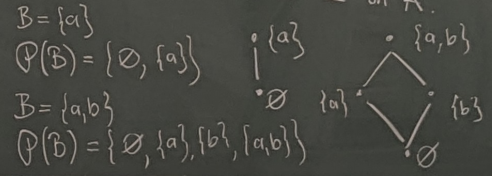
\includegraphics[width=0.7\linewidth]{images/poset.png}
    \end{figure}
\end{example}
\begin{definition}
    \begin{itemize}
    \item Let $(A,\sqsubseteq)$ be a poset. A function $F$ from $A$ to $A$ is \textbf{monotone} (order-preserving, homomorphism) if for all $x$ and $y$ in $A$, if $x \sqsubseteq y$, then $F(x) \sqsubseteq F(y)$.
    %
    \item $F$ has a fixpoint $x$ in $A$ if there exists $x$ in $A$ such that $F(x)=x$. 
    \item $x$ in $A$ is a pre-fixpoint of $F$ if $x \sqsubseteq F(x)$ and is a post-fixpoint of $F$, if $F(x) \sqsubseteq x$. 
    \end{itemize}
\end{definition}
\begin{definition}
    Let $(A,\sqsubseteq)$ be a poset.
    \begin{itemize}
        \item $x$ in $A$ is an \textbf{upper bound}(lower bound) on a subset $B$ of $A$ if for all $y$ in $B$, it holds that $y \sqsubseteq x$ ($x \sqsubseteq y$).
        \item $x$ is the least upper bound of $B$ if (i) $x$ is an upper bound of $B$ and (ii) for all upper bounds $y$ of $B$, we have $x \sqsubseteq y$. We denote such $x$ by $\bigsqcup B$.
        \item $x$ is the greatest lower bound of $B$ if (i) $x$ is a lower bound of $B$ and (ii) for all lower bounds $y$ of $B$, we have $y \sqsubseteq x$. We denote such $x$ by $\bigsqcap B$.
    \end{itemize}
\end{definition}
\begin{example} 
    \begin{itemize}
        \item Consider the poset $(\N,\leq)$. Then for any $B \subseteq \N$, if $B$ is finite, $\bigsqcup B$ is well-defined and equal to $\max B$. If $B$ is infinite, then $\bigsqcup B$ does not exist. 
        \item Consider the poset $(\N \cup \{\infty\},\leq)$ where for all $x$ in $\N$, it holds that $x \leq \infty$. Then for all $B \subseteq \N$, the least upper bound $\bigsqcup B$ is well-define. 
        \item Let $A$ be any set and consider the poset $(\P(A),\subseteq)$. For any subset $B$ of $\P(A)$, it holds that $\bigsqcup B = \bigcup B$ and $\bigsqcap B = \bigcap B$. 
    \end{itemize}
\end{example}
\begin{definition}
    Poset $(A,\sqsubseteq)$ is a \textbf{complete-lattice} if for all $B \subseteq A$, both $\bigsqcap B$ and $\bigsqcup B$ exist.
\end{definition}
\begin{example}
    Let $(A,\sqsubseteq)$ be a complete-lattice. 
    \begin{itemize}
        \item $\bigsqcup A = \top$
        \item $\bigsqcap A = \bot$
        \item $\bigsqcup \varnothing = \bot$
        \item $\bigsqcap \varnothing = \top$
    \end{itemize}
\end{example}
\begin{theorem}[Knaster-Tarski]
    For every complete lattice $(A,\sqsubseteq)$ and monotone function $F$ on $A$, it holds that
    \begin{enumerate}
        \item $\bigsqcup \{x\in A| x \sqsubseteq F(x)\}$ is the unique greatest fixpoint of $F$. 
        \item $\bigsqcap \{x \in A| F(x) \sqsubseteq x\}$ is the unique least fixpoint of $F$. 
    \end{enumerate}
\end{theorem}


\begin{homework}
    Prove the Knaster Tarski Theorem.
\end{homework}

 